%% Exemplo de uso da versão da classe  _eesc-stt.cls_, uma adaptação 
%% para o Programa de Engenharia de Transportes da EESC-USP
%% da classe _eesc.cls_, do PPG-EEC da EESC, feita por Athila e Monaro.
%% A classe _eesc.cls_ é uma customifsdffdsfzação da classe abntex2.cls, feita
%% pelo abntex2 group (http://abntex2.googlecode.com/)
%%
%% Customização da classe eesc.cls feita por setti@sc.usp.br
%% 
%% ------------------------------------------------------------------------
%% eesc-stt.cls: classe para elaboração de tese de doutorado, dissertação de
%% mestrado e texto para qualificação (mestrado e doutorado) em conformidade com 
%% a norma ABNT NBR 14724:2011, adequada às exigências da CPG-EESC, para o 
%% Programa de Pós-Graduação em Engenharia de Transportes. 
%% ------------------------------------------------------------------------

\documentclass[qualimst]{eesc-stt}

\usepackage[utf8]{inputenc}
\usepackage[T1]{fontenc}

% ------------------------------------------------------------------------
% Opções da classe eesc-stt.cls:
% 	tesedr:     Formata documento para tese de doutorado
%	qualidr:    Formata documento para qualificação de doutorado
% 	dissertmst: Formata documento para dissertação de mestrado
% 	qualimst:   Formata documento para qualificação de mestrado
% ------------------------------------------------------------------------
 
% Packages usados na classe eesc-stt.cls
% Esses packages são definidos em abntex2.cls e eesc-stt (que não devem ser modificado sem mudar de nome)
% A folha é A4 e as margens são definidas de acordo com a NBR 14724:2011

%% ---
%% Escolha da tipologia usada no documento
%%
%% (apenas fontes com símbolos matemáticos são listadas aqui)
%% Nota: escolha apenas uma tipologia, apagando os % das linhas desejadas
%% --- 
 
% ---
%
% ---

% ---
% Definições da tipologia usada
% (apenas fontes com símbolos matemáticos são listadas aqui)
% Nota: escolha apenas uma tipologia, apagando os % das linhas desejadas
% ---


% Usa a fonte Latin Modern (versão ampliada de CM, a tradicional do LaTeX)
%\usepackage{lmodern}			

% Usa a fonte Charter para texto, Inconsolata para tt e Cabin para sans serif
%\usepackage[scaled=.98,sups]{XCharter}% lining figures in math
%\usepackage[scaled=1.04,varqu,varl]{zi4}% inconsolata typewriter
%\usepackage[type1]{cabin}% sans serif
%\usepackage[libertine,bigdelims,scaled=1.07]{newtxmath}


% Usa a fonte Linux Libertine e Biolinum
\usepackage[tt=true,sb=true]{libertine}
\usepackage[libertine,bigdelims]{newtxmath}

% Usa a fonte Bera (versão de Vera Serif}
%\usepackage{bera}

% Usa a fonte Vera Sans (sem serifa)
%\usepackage{arev}


% Usa a fonte Kerkis (versão de Bookman)
%\usepackage{kmath,kerkis} %  Nessa ordem, kmath muda a fonte do texto

% Usa a fonte Baskervald (versão de Baskerville, serifa), Linux Biolinum (sem serifa) e SourceCodePro (tt)
%\usepackage[lf]{Baskervaldx} % lining figures
%\usepackage{biolinum}% sans serif
%\usepackage[regular,bold,light,scaled=.8785,lf]{sourcecodepro}
%\usepackage[bigdelims,vvarbb]{newtxmath} % math italic letters from Times
%\usepackage[cal=boondoxo]{mathalfa} % mathcal from STIX, unslanted a bit
%\renewcommand*\oldstylenums[1]{\textosf{#1}}

% Usa a fonte Computer Bright (sem serifa)
%\usepackage{cmbright}

% Usa a font Stix (semelhante a Times New Roman)
%\usepackage{stix}

% Usa a fonte Utopia com o MathDesign
%\usepackage[adobe-utopia]{mathdesign}
 
% Usa a fonte URW Palladio (Palatino)
%\usepackage[sc]{mathpazo}
%%--
%% Final da definição da tipologia
%%--


\usepackage{amsmath}

%% ---
%% Packages para processamento de componentes deste documento (tese-stt.tex)  
%% ---
\usepackage{cmap}				% Mapeia caracteres especiais, necessário para criar um searchable PDF
%\usepackage{makeidx}            % Cria o indice remissivo (descomente se for usar um índice remissivo)
 	% para mais detalhes, estude makeindex.pdf, no CTAN
\usepackage{hyperref}  			% Controla a formação do links no pdf e hyperlinks
 	% para mais detalhes, estude hyperref.sty, no CTAN
\usepackage{lastpage}			% Usado para inserir a Ficha catalográfica no lugar certo (eesc.cls)
%\usepackage{nomencl} 			% Cria a lista de simbolos (descomente se for usar lista de símbolos)
 	% para mais detalhes, estude nomencl.pdf, no CTAN
\usepackage{graphicx}			% Usado para incluir os arquivos pdf com as figuras e gráficos
 	% veja exemplo de inclusão de figuras neste documento
%% ---
%% Final dos packages para processamento de componentes do texto  
%% ---
 

% ---
% Pacotes adicionais, usados apenas no âmbito do modelo eesc.cls 
% ---
%\usepackage[printonlyused]{acronym}	% Cria lista de siglas (descomente se for usar lista de siglas)
\usepackage[table]{xcolor}				% Facilita o uso de cores
% --- fim dos pacotes adicionais do eesc.cls


%
% Pacote para geração de texto para encher linguiça (lorem ipsum)
% Apague essas linhas quando estiver fazendo o arquivo da sua tese/dissertação
\usepackage{lipsum}				       % para geração de dummy text

 

% ---
% Dados para a montagem da CAPA e da FOLHA DE ROSTO
% ---
%
% \titulo - comando para entrar com o título em português e inglês
% 			parâmetros são usados em diversos locais do documento
% Uso: \titulo{Título em Português}{Title in English}

\titulo{Dados online mudei}
	   {Very long title in English, full of letters, taking a lot of space}
%
% \autor	comando para entrar com o nome do autor
% 			parâmetros são usados em diversos locais do documento
% Uso: \autor{Nome Completo do Autor}{Sobrenome, N.~M.}
 
\autor{Quasímodo Affonso Barbalho Nogueira da Cunha}{Cunha, Q.~A.~B.~N.}
%
 
% \cidade	comando para entrar com o nome da cidade
% 			parâmetro é usado em diversos locais do documento
\local{São Carlos}

% \data		comando para entrar com o ano da defesa
\data{2014}

% \areaconcentracao		comando para definir a área de concentração
%						PPG-ET: 	Infraestrutura de Transportes ou 
%									Planejamento e Operação de Sistemas de Transportes
%
\areaconcentracao{Planejamento e Operação de Sistemas de Transportes}

% \orientador		comando para entrar com nome do orientador
\orientador{Prof.~Dr.~José Reynaldo Setti}

% \coorientador		comando para entrar com nome do coorientador (só doutorado na USP)
\coorientador{Prof. Dr. Ing. Paulaner Delikatt Zömfflig}
% ---

%%------------
%% Processamento do índice remissivo e da lista de siglas
%%    Nota: como não é usual fazer índice remissivo e lista de siglas
%%    no PPG-ET, as linhas e respectivos pacotes(\includepackage)
%%	  para criação do índice remissivo e da LdeS foram comentadas
%%------------
 	
% ---
% compila o indice remissivo (descomente essa linha e o package makeidx)
% ---
%\makeindex
% ---

	
% ---
% Compila a lista de abreviaturas e siglas 
% ---
%	Para construir as entradas da lista de abreviaturas, consulte
%	a documentação do abnTeX2
%
% 	Descomente a linha a seguir para compilar a lista de siglas
% ---
%\makenomenclature
% ---

%-------
% Inserção da ficha catalográfica no verso da folha de rosto
%-------
	%
	% \inserirfichacatalografica	comando para inserir ficha catalográfica
	% Uso: \inserirfichacatalografica{nomedoarquivo.pdf}
	%
	% Caso o comando \inserirfichacatalografica seja definido, a ficha catalográfica
	% será inserida atrás da folha de rosto. Caso contrário a página será deixada em
	% branco.
	% Escaneie a ficha catalográfica da biblioteca num arquivo pdf
	%
	% CUIDADO: Esta opção deve ser preenchida antes do comando \maketitle
	% ---
%\inserirfichacatalografica{fichaCatalografica.pdf}
% ---

%-------
% Inserção da folha de aprovação depois da folha de rosto
% ------
	%
	% \inserirfolhaaprovacao	comando para inserir folha de aprovação
	% Uso: \inserirfolhaaprovacao{nomedoarquivo.pdf}
	%
	% Caso o comando \inserirfolhaaprovacao seja definido, a a folha de aprovação
	% será inserida. Além disso, conforme Resolução CoPGr 5890, as informações 
	% de rodapé são inseridas apropriadamente na folha de rosto, informando que 
	% esta versão é uma versão corrigida e que a versão de defesa está arquivada
	% no SVPOSGR-EESC.
	% Escaneie a folha de aprovação feita pela secretaria do PPG-ET num arquivo pdf
	%
	% CUIDADO: Esta opção deve ser preenchida antes do comando \maketitle
% ---
%\inserirfolhaaprovacao{folhaAprovacao.pdf}
% ---


%-----------------
%	Design dos títulos dos capítulos
%-----------------
%
% abntex2.cls e eesc.cls usam uma das alternativas do memoir.cls, sem dar chance  
% de escolha para o usuário. O design escolhido é feio, na minha opinião.
% O design dos títulos dos capítulos a seguir pode ser usado para substituir o
% padrão do memoir.cls. É possível modificar a cor da caixa (ChapBlue) e da
% fonte com o número do capítulo (ChapWhite) e a posição da caixa (à direita
% ou à esquerda).
% Se você não quiser usar esse design para os títulos dos capítulos e  
% preferir usar o design do abntex2.cls, basta comentar a linha com o
% comando \chapterstyle{...}
%
\definecolor{ChapWhite}{rgb}{1,1,1}					% Para trocar a cor, mude os valores de {1,1,1} (branco)
\newcommand{\LargeFont}{% Needs a 'stretchable' font
      \usefont{\encodingdefault}{\sfdefault}{b}{n}%
      \fontsize{60}{80}\selectfont\color{ChapWhite}}
\newsavebox{\ChpNumBox}
\definecolor{ChapBlue}{rgb}{0.65,0.25,0.35}			% Para trocar a cor, mude os valores de {.65,.25,.35}
\makeatletter
\newcommand*{\thickhrulefill}{%
  \color{ChapBlue}\leavevmode\leaders\hrule height 1\p@ \hfill \kern%  
  \z@\color{black}}
\newcommand*\BuildChpNum[2]{%
  \begin{tabular}[t]{@{}c@{}}
    \makebox[0pt][c]{#1\strut}  \\[.5ex]
    \colorbox{ChapBlue}{%
      \rule[-10em]{0pt}{0pt}%
      \rule{1.3ex}{0pt}\color{black}#2\strut
      \rule{0.15ex}{0pt}}%
  \end{tabular}}
%--
% GreyBoxRight faz o título do capítulo ficar alinhado à esquerda
%--
\makechapterstyle{GrayBoxRight}{%
  \renewcommand{\chapnamefont}{\large\sffamily\bfseries}
  \renewcommand{\chapnumfont}{\LargeFont}
  \renewcommand{\chaptitlefont}{\raggedleft\Huge\sffamily\bfseries}
  \setlength{\beforechapskip}{20pt}
  \setlength{\midchapskip}{26pt}
  \setlength{\afterchapskip}{40pt}
  \renewcommand{\printchaptername}{}
  \renewcommand{\chapternamenum}{}
  \renewcommand{\printchapternum}{%
    \sbox{\ChpNumBox}{%
      \BuildChpNum{\chapnamefont\@chapapp}%
      {\chapnumfont\thechapter}}}
  \renewcommand{\printchapternonum}{%
    \sbox{\ChpNumBox}{%
      \BuildChpNum{\chapnamefont\vphantom{\@chapapp}}%
      {\chapnumfont\hphantom{\thechapter}}}}
  \renewcommand{\afterchapternum}{}
  \renewcommand{\printchaptertitle}[1]{%
    \parbox[t]{\hsize-\wd\ChpNumBox-1em}{%
      \vspace{\midchapskip}%
      \thickhrulefill\par
     		\chaptitlefont ##1}%
    \hfill\usebox{\ChpNumBox} % põe a caixa na direita
	}%
}% fecha \makechapterstyle{GrayBoxRight}
%--
% GreyBoxLeft faz o título do capítulo ficar alinhado à esquerda
%--
\makechapterstyle{GrayBoxLeft}{%
  \renewcommand{\chapnamefont}{\large\sffamily\bfseries}
  \renewcommand{\chapnumfont}{\LargeFont}
  \renewcommand{\chaptitlefont}{\raggedright\Huge\sffamily\bfseries}
  \setlength{\beforechapskip}{20pt}
  \setlength{\midchapskip}{26pt}
  \setlength{\afterchapskip}{40pt}
  \renewcommand{\printchaptername}{}
  \renewcommand{\chapternamenum}{}
  \renewcommand{\printchapternum}{%
    \sbox{\ChpNumBox}{%
      \BuildChpNum{\chapnamefont\@chapapp}%
      {\chapnumfont\thechapter}}}
  \renewcommand{\printchapternonum}{%
    \sbox{\ChpNumBox}{%
      \BuildChpNum{\chapnamefont\vphantom{\@chapapp}}%
      {\chapnumfont\hphantom{\thechapter}}}}
  \renewcommand{\afterchapternum}{}
% --
% caixa na direita e título e alinhado à esquerda
% --
  \renewcommand{\printchaptertitle}[1]{%
    \usebox{\ChpNumBox}\hfill % linha original
    \parbox[t]{\hsize-\wd\ChpNumBox-1em}{%
      \vspace{\midchapskip}%
      \thickhrulefill\par
      \chaptitlefont ##1\par}}%
}% fecha \makechapterstyle{GrayBoxLeft}
%--
% Final do design dos títulos dos capítulos
%--
 	
%--
% Escolha do tipo de design dos títulos dos capítulos:
% Opções:
% GreyBoxLeft  - caixa na esquerda e texto alinhado à esquerda
% GreyBoxRight - caixa na direita e texto alinhado à direita
%--
%	Comente a linha a seguir se for usar o design do abntex2.cls
\chapterstyle{GrayBoxRight}

%%------------
%	Correção da numeração de tabelas, figuras e equações
%
%	abntex2.cls numera tabelas, figuras e equações, por definição
%   como Figura 1 ao invés de Figura {chapternum}{fignum}.
%	(deve ser por causa de alguma NBR imbecil)
%	Para corrigir esse defeito, as linhas a seguir mudam a forma
%	de numerar para a mais inteligente e usual em teses.
%	Se você preferir seguir a ABNT ao pé da letra, comente as
%   linhas a seguir
\counterwithin{figure}{chapter}
\counterwithin{table}{chapter}
\counterwithin{equation}{chapter}

%%-------------
%	Definição do símbolo usado na lista itemize
%   (se desejar manter o quadrado com sombra etc., comente ou apague as linhas a seguir
\renewcommand{\labelitemi}{$\bullet$}
\renewcommand{\labelitemii}{\footnotesize$\blacktriangleright$}
\renewcommand{\labelitemiii}{$\circ$}
\renewcommand{\labelitemiv}{$\triangleright$}

% ----
% Início do documento
% ----

\begin{document}

% ----------------------------------------------------------
% ELEMENTOS PRÉ-TEXTUAIS
% ----------------------------------------------------------
\pretextual

% ---
% AbnTeX2 redefine o comando \maketitle para que ele faça as seguintes tarefas:
%	- elaboração da capa e do seu verso (em branco); 
%	- elaboração da folha de rosto 
%	- inserção do arquivo PDF com a ficha catalográfica (se existir), no verso da folha de rosto; e 
%	- inserção da folha de aprovação (se existir).
% ---
\maketitle


% ---
%  Dedicatória
% ---
% \imprimirdedicatoria		comando para imprimir a dedicatória (opcional)
% Uso: \imprimirdedicatoria{texto da dedicatória}
% ---
\imprimirdedicatoria{Use o comando \emph{\texttt{\textbackslash{}imprimirdedicatória\{...\}}}
	para colocar sua dedicatória numa nova página. \\
	Para quebrar a linha, use \emph{\texttt{\textbackslash\textbackslash}},
	pois linhas em branco gerarão mensagens de erro.
	Dedicatórias de mais de uma linha ficam ``feias'', já o texto é sempre centralizado, por definição.\\ 
	\hspace*{1pt}\\
	Ao meu avô, \\
	À memória da minha avó, \\
	Ao meu pai, \\ À minha adorada mãezinha, \\
	E, finalmente, aos meu onze irmãos e irmãs.\\
	Sem vocês, isso seria muito mais curto!
}% ---

% ---
% Agradecimentos
% ---
\imprimiragradecimentos{
Os agradecimentos são colocados usando-se o ambiente 
\texttt{\textbackslash{}imprimiragradecimentos\{...\}}. 

Como os agradecimentos são um capítulo sem numeração, é possível colocar mais de 
um parágrafo de agradecimentos. Basta usar uma 
linha em branco entre os blocos de texto e o próprio \LaTeX{} cuidará de 
fazer a composição tipográfica correta.
}
% ---

% ---
% Epígrafe
% ---
\imprimirepigrafe{
	``É completamente incompreensível o interesse em torno deste\\ 
	assunto depois de tantos milhares de anos de uso.''\\
		\emph{(Millor Fernandes)}\\ \vspace{16pt} 
	De acordo com os dicionários, epígrafe é ``fragmento de texto, citação curta,  
	máxima etc., colocada em frontispício de livro, no início de uma narrativa, 
	um capítulo etc.'' e serve de tema ao assunto, 
	para resumir o sentido ou  ainda para situar a motivação da obra.\\ \vspace{16pt}
	Use o ambiente 
	\emph{\texttt{\textbackslash{}imprimirepigrafe\{...\}}} para colocar a 
	epígrafe na sua tese ou dissertação. 	
	Use \emph{\texttt{\textbackslash\textbackslash}}
	para quebrar linhas, pois linhas em branco gerarão mensagens de erro.\\
	Use \emph{\texttt{\textbackslash{}vspace\{16pt\}}} para dar espaço entre
	parágrafos.
}
% ---

% ---
% RESUMO e ABSTRACT
% ---

% Resumo em português
\begin{resumo}{Palavra-chave 1. Palavra-chave 2. Palavra-chave 3}
     Use o ambiente \texttt{resumo} para inserir o resumo do trabalho. Este
 	 ambiente irá gerar uma página como esta, com a referência bibliográfica
 	 para citação, o texto do resumo e, ao final, as palavras-chaves.
 	 
 	 Para fornecer as palavras-chaves, inclua-as entre \texttt{\{} e \texttt{\}},
 	 logo após \verb|\begin{resumo}|.  Elas devem estar 
 	 separadas entre si por ponto, como em \\
 	 \hspace*{1em}\verb|\begin{resumo}{Palavra-chave 1. Palavra-chave 2}|\\
 	 \hspace*{2em}\verb|Blá, blá, blá...|\\
 	 \hspace*{1em}\verb|\end{resumo}|\\
 	 Não há ponto depois da última palavra-chave, pois o ambiente 
 	 \texttt{resumo} já o inclui automaticamente. Se houver um ponto depois
 	 da última palavra-chave, aparecerão dois pontos finais no seu documento,
 	 como em\\
 	 \hspace*{5em}\textcolor{red}{\textsf{\textbf{Palavras-chave}: Palavra1. Palavra2\textbf{..}}}\\ 
 	 Para entender melhor, consulte o arquivo usado para gerar este documento.
 	 
 	 No ambiente  \texttt{resumo}, pode-se usar linhas em branco para separar os parágrafos,
 	 pois o Resumo é um capítulo sem numeração. \vspace{-12pt}

\end{resumo}

% Resumo em inglês
\begin{abstract}{Keyword 1. Keyword 2. Keyword 3}
	To insert the abstract, use the \texttt{abstract} environment. A page like this,
	starting with the bibliographic reference, followed by the text and by the list of
	keywords will be created in the document.
	
	 Use  \texttt{abstract}  exactly the same way you would use \texttt{resumo}.
	
\end{abstract}
% ---

% ---
% Inserir lista de figuras
%
% o comando \listailustracoes do abntext2 deve ser usado no lugar 
% do comando \listoffigures do LaTeX
% ---
\listailustracoes
% ---

% ---
% Inserir lista de tabelas
%
% o comando \listatabelas do abntext2 deve ser usado no lugar
% do comando do LaTeX \listoftables
% ---
\listatabelas
% ---

% ---
% Inserir lista de abreviaturas e siglas (opcional), 
% descomente se for usar, incluindo linhas comentadas anteriormente
% ---
%\listasiglas{abrev/Abreviaturas}
% ---

% ---
% Inserir o sumário (índice de matéria)
%
% abntext2 obriga o uso do comando \sumario no lugar do
% comando LaTeX \tableofcontents
% ---
\sumario
% ---

% ----------------------------------------------------------
% ELEMENTOS TEXTUAIS
% ----------------------------------------------------------
\mainmatter

%-------
% Use o comando \include para incluir os capítulos da tese/dissertação
% cada arquivo será incluído numa nova página
%
%	Não use acentos ou cedilha ou espaços em branco nos nomes dos arquivos
%   use / no lugar de \, como em: {cap_intro/introducao} no lugar de {cap_intro\introducao}
%   . representa o diretorio atual -- {./cap1/capitulo_1}


% !TEX encoding = ISO-8859-1	
% Define o encoding do arquivo (TeXworks e TeXstudio?) para que os acentos possam ser
% usados diretamente: é e não \'e

\chapter{Introdução}

Este documento que simula parte de uma tese de doutorado foi elaborado para facilitar o uso da
classe \texttt{\abnTeX.cls}\ na elaboração de teses e dissertações no \textbf{Programa de Pós-Graduação
em Engenharia de Transportes}, da EESC-USP, usando a classe customizada \texttt{eesc-stt.cls}. 

Esta customização para o PPG-ET foi criada a partir da classe \texttt{eesc.cls},
por sua vez também uma customização da classe \texttt{\abnTeX.cls}, feita por Athila Quaresma Santos e Renato Monaro,   
para atender às exigências da CPG-EESC (mais especificamente, do Programa de 
Pós-Graduação em Engenharia Elétrica e de Computação da EESC). 

A classe \texttt{\abnTeX.cls} é uma adaptação da classe \texttt{memoir.cls} para as 
(muitas vezes inexplicáveis) exigências da NBR-14724:2011 \emph{Informação 
e documentação -- Trabalhos acadêmicos -- Apresentação} e suas diversas ``irmãs''. A classe \texttt{\abnTeX.cls} requer o uso do 
o pacote \texttt{abntex2cite.sty} para gerar a
bibliografia e as citações bibliográficas ao longo do texto em conformidade
com a norma NBR-10520:2002 \cite{NBR10520:2002}.
 
Lendo este documento e os comentários colocados ao longo do seu código-fonte, 
você poderá familiarizar-se com o uso da classe \texttt{eesc-stt.cls} e do pacote 
\texttt{abntex2cite} e aprender como usar o \LaTeX\ em algumas situações comuns
durante a elaboração de uma tese/dissertação. Em pontos apropriados do texto, há
links clicáveis para documentação mais completa ou, pelo menos, indicação da 
sua existência no CTAN (Comprehensive \TeX\ Archive Network) -- 
\href{http://www.ctan.org/pkg/abntex2}{\fbox{link para CTAN.org}}.

Você pode gerar este pdf processando o arquivo \texttt{tese-stt.tex} no \LaTeX.

% !TEX encoding = ISO-8859-1

%% Material derivado de:
%% abntex2-modelo-include-comandos.tex, v-1.4 laurocesar
%% Copyright 2012-2013 by abnTeX2 group at http://abntex2.googlecode.com/ 
%%
%% This work may be distributed and/or modified under the
%% conditions of the LaTeX Project Public License, either version 1.3
%% of this license or (at your option) any later version.
%% The latest version of this license is in
%%   http://www.latex-project.org/lppl.txt
%% and version 1.3 or later is part of all distributions of LaTeX
%% version 2005/12/01 or later.
%%

% ---
% Este capítulo, utilizado por diferentes exemplos do abnTeX2, ilustra o uso de
% comandos do abnTeX2 e de LaTeX.
% ---
 
\chapter{Uso de nada do \protect{\LaTeX} e da classe abn\protect{\TeX}2}
\label{cap_exemplos}

%\chapterprecishere{Isto é uma sinopse de capítulo. A ABNT não 
%normatiza esse tipo de resumo, que não deve ser usado
%numa tese.  Use o comando 
%\emph{\texttt{\textbackslash{}chapterprecishere\{...\}}} para inserir a
%sinopse num documento.
%}\index{sinopse de capítulo}


É perfeitamente possível e, quiçá, até melhor, escrever uma 
tese ou dissertação sem usar nenhum dos comandos e ambientes 
da classe {abn\TeX{}2}, com exceção daqueles do pacote 
\texttt{abntex2cite.sty}, como \verb|\citeonline{..}|. 
Este capítulo mostra como usar alguns dos comandos do \LaTeX\ e 
comandos específicos da classe {abn\TeX{}2} que podem ser úteis na
preparação do seu documento. 

% ---
\section{Citações diretas e aforismos}
% ---

\index{citações!diretas}A classe {abn\TeX{}2} define o ambiente \texttt{citacao} para incluir
citações diretas com mais de três linhas, conforme normatizado na NBR10520 \cite{NBR10520:2002}:
\begin{citacao}
As citações diretas, com mais de três linhas, são
destacadas com recuo de 4 cm da margem esquerda, com letra menor que a do texto
e sem as aspas. Em documentos datilografados, deve-se
observar apenas o recuo (só a ABNT ainda usa máquina de escrever!) \cite[5.3]{NBR10520:2002}. 
\end{citacao}
O resultado é, sem sombra de dúvida, um insulto à tipografia de qualidade 
-- veja, por exemplo \citeonline[p.~17--18, 41]{bring04}.
Por isso, procure usar o ambiente do \LaTeX\ \texttt{quotation} para citações longas
e \texttt{quote} para aforismos e frases curtas. Nenhuma pessoa de sã
consciência vai se lembrar da NBR10520, de qualquer forma.   
Veja como uma citação fica muito melhor usando o ambiente \texttt{quotation}:
	\begin{quotation}\itshape
	As citações diretas com o ambiente \texttt{quotation} são
	destacadas com recuo de ambas as margens. 
	Se desejar usar letra menor que a do texto,
	utilize o comando \upshape{\verb|\small|}\itshape, logo após \upshape\verb|\begin{quotation}| \cite[p.~26]{LaTeX}.
	\end{quotation}

Citações curta podem aparecer entre aspas: ``A diferença entre a galinha e o político é 
que o político cacareja e não bota o ovo.'' (Millor Fernandes). Ou usando o ambiente \verb|quote|:
	\begin{quote}
	A diferença entre a galinha e o político é que 
	o político cacareja e não bota o ovo.
	\emph{Millor Fernandes}
	\end{quote} 

% ---
\section{Remissões internas}
% ---

Quando se faz referência no texto à Tabela~\ref{tab-aderencia}, têm-se um exemplo de remissão interna,
que também pode ser feita quando indicamos o \autoref{cap_exemplos}\footnote{O
número do capítulo indicado é
\ref{cap_exemplos}, que se inicia à página \pageref{cap_exemplos}.}
(\nameref{cap_exemplos}, \autopageref{cap_exemplos}), por exemplo.

Remissões internas ajudam o leitor a encontrar informação na tese. Notas de 
rodapé, por sua vez, confundem mais do que ajudam e dão a impressão de que você
se esqueceu de incluir algo no texto e, ao relê-lo, ficou com 
preguiça de reescrever todo o parágrafo e resolveu ``colar'' aquela informação
no rodapé da página. Por isso, evite a todo custo usar notas de rodapé.

% ---
\section{Tabelas}
% ---

\index{tabelas}A Tabela~\ref{tab-aderencia} é um exemplo de tabela construída em
\LaTeX, usando-se o pacote \verb|booktabs.sty|. Para aprender a usá-lo melhor, refira-se à documentação disponível no CTAN. 

Note que o \LaTeX\ posiciona os \emph{floats} 
(figuras ou tabelas) no topo ou no pé da página, porque esses elementos devem ``flutuar''
no documento e serem posicionados em locais convenientes \cite[p.~59]{LaTeX}. Com isso, costumam
ser colocados no topo (ou pé) da página seguinte à em que são mencionados pela 
primeira vez no texto. 

Pode-se usar uma outra família de fontes, como a sem serifa, para distinguir melhor a tabela
do texto do documento. Para fazer isso, inclua o comando \verb|\sffamily| antes de qualquer
texto da tabela (isso não altera o texto que aparece na lista de tabelas, que vai 
ser composto usando tipos com serifa).  A Tabela~\ref{tab-aderencia-rm} permite que você
compare os dois estilos e escolha o que mais lhe agradar.

As Tabelas~\ref{tab-aderencia} e \ref{tab-aderencia-rm} também ilustram o uso 
do ambiente \verb|minipage| para colocar duas ou mais tabelas ou figuras dentro
de um \emph{float}. Para aprender a fazer figuras e tabelas mais complexas,
consulte \emph{Using Imported Graphics in \protect{\LaTeX} and pdf\protect{\LaTeX}} \cite{epslatex06}, disponível no CTAN.

\begin{table}
\begin{minipage}[t]{72mm}\centering\sffamily
  {\caption[Valores da aderência $f$ para diversos estados do trilho] 
  		{Valores da aderência $f$ para diversos estados do trilho \cite{hay82}\label{tab-aderencia}}}
	%\vspace{4pt}
    {\footnotesize % usado para deixar as letras da tabela do mesmo tamanho das letras do caption
\begin{tabular}{ll} \toprule
  \textbf{\textit{Estado do trilho}} & \textbf{\textit{Aderência}} $f$ \\ \midrule
  Totalmente seco e limpo & 0,33 \\
  Lavado pela chuva       & 0,33 \\
  Seco e limpo            & 0,22 \\
  Seco e sujo             & 0,20 \\
  Úmido de orvalho        & 0,125 \\
  Úmido e sujo            & 0,11 \\
  Sujo com óleo           & 0,10 \\ \bottomrule
\end{tabular}}
\end{minipage}
\hfill
\begin{minipage}[t]{75mm}\centering\rmfamily
  \caption{Mesma tabela, com a mesma letra do texto \label{tab-aderencia-rm}}
	%\vspace{4pt}
    {\footnotesize % usado para deixar as letras da tabela do mesmo tamanho das letras do caption
\begin{tabular}{ll} \toprule
  \textbf{\textit{Estado do trilho}} & \textbf{\textit{Aderência}} $f$ \\ \midrule
  Totalmente seco e limpo & 0,33 \\
  Lavado pela chuva       & 0,33 \\
  Seco e limpo            & 0,22 \\
  Seco e sujo             & 0,20 \\
  Úmido de orvalho        & 0,125 \\
  Úmido e sujo            & 0,11 \\
  Sujo com óleo           & 0,10 \\ \bottomrule
\end{tabular}}
\end{minipage}
\end{table}


% ---
\section{Equações e expressões matemáticas}
% ---

\index{expressões matemáticas}Use o ambiente \texttt{equation} para escrever
equações  numeradas:
\begin{equation}
  x = \frac{-b \pm \sqrt{b^2-4ac}}{2a}.
\end{equation}
Também é possível usar colchetes para escrever uma expressão
matemática que não é numerada:
\[
\left|\sum_{i=1}^n a_ib_i\right|
\le
\left(\sum_{i=1}^n a_i^2\right)^{1/2}
\sqrt{\sum_{i=1}^n b_i^2}
\]

Às vezes, é preciso definir as variáveis e parâmetros de uma equação, 
como:
    \begin{equation}
    R_{r} = ( c_{1} + c_{2} \, V) \, G,
    \label{e3:3}
    \end{equation}
\begin{tabbing}
   em que \hspace{1em}
   \=$R_{r}$:  \hspace{2.3em}  \=resistência de rolamento [N] \\
   \>$V$:   \> velocidade do veículo [km/h]; \\
   \>$G$:   \> peso do veículo [kN]; e \\
   \>$c_1$ e $c_2$: \> constantes.
\end{tabbing}
Para isso, use o ambiente \texttt{tabbing}. Consulte o arquivo
usado para gerar o texto deste capítulo para um exemplo. Acima de 
tudo, lembre-se de que \emph{onde} só deve ser usado para se 
referir a locais geográficos; use \emph{em que}, \emph{na qual} etc.
para se referir à \autoref{e3:3}.

Numa linha de comando de texto, expressões matemáticas são colocadas en
\verb|$...$|, como em $ \lim_{x \to \infty} e^{-x} = 0 $, para que 
fiquem na mesma linha. Note que as variáveis numa
equação \emph{sempre} aparecem em itálico, mas números e funções matemáticas,
não. Além disso, não use itálico para escrever variáveis
no texto (e vice-versa), pois há diferenças visíveis entre o espaçamento 
no modo matemático (\verb|$...$|) e no itálico (\verb|\emph{...}|), além
do uso correto dos símbolos e sinais matemáticos. 
Use \verb|$y = x-1$| para escrever $y = x-1$ no texto,
ao invés de \emph{y = x-1}, obtido usando-se \verb|\emph{y = x-1}|.

Consulte um manual do \LaTeX\ para mais informações sobre como
escrever corretamente expressões matemáticas -- afinal de contas,
Donald Knuth criou o \TeX\ para tipografar matemática corretamente
\cite[p.~xiii]{LaTeX}.

\section{Figuras}

\index{figuras}Apesar de ser possível criar figuras diretamente em \LaTeX,
como o exemplo da \autoref{fig_circulo}, você certamente não vai querer 
fazer isso. O processo é insanamente tedioso e requer a entrada das
coordenadas $(x,y)$ iniciais e outras informações de todos as linhas
do gráfico.  

\begin{figure}
	\begin{center}
	    \setlength{\unitlength}{4cm}
		\begin{picture}(2,1)\thicklines
		\put(0,0){\vector(0,1){1}}
		\put(0,0){\vector(1,0){2}}
		\put(1.85,-.1){\footnotesize\emph{x}}
		\put(-.1,.85){\footnotesize\emph{y}}
		\linethickness{0.5mm}
		\qbezier(0,0)(0.5,0)(1,.5)
		\qbezier(1,0.5)(1.25,.9)(1.8,0.9)
		\end{picture}
	\end{center}
	\caption{Um gráfico desenhado com comandos do \protect{\LaTeX}}
	\label{fig_circulo}
\end{figure}
\begin{figure}\sffamily
	\begin{center}
	    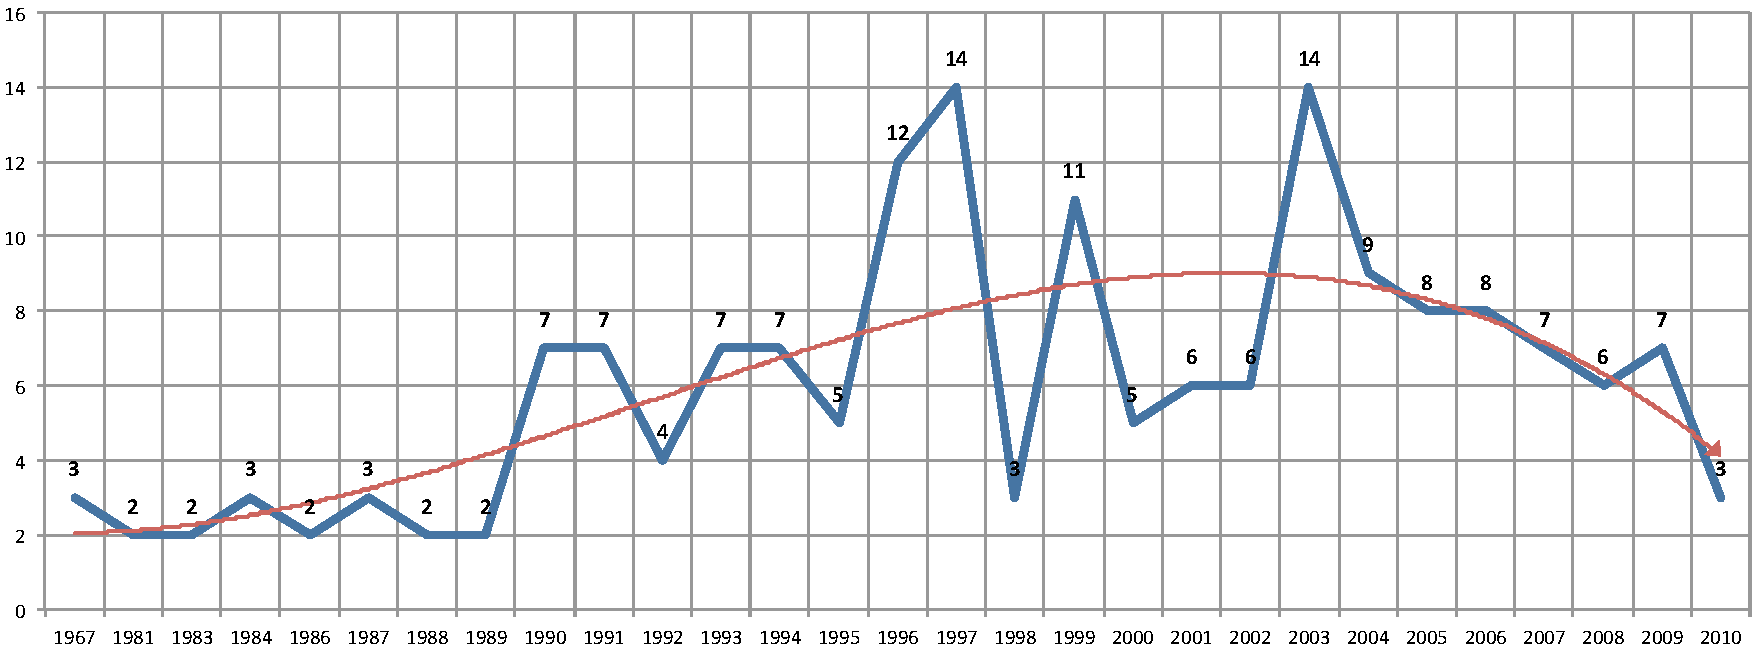
\includegraphics[width=160mm]{cap1/abntex2-img-grafico.pdf}
	\end{center}
	\caption[Gráficos feitos em Excel devem ser gravados como PDF para serem
	usados em \protect{\LaTeX}...]
	{Gráficos feitos em Excel devem ser gravados como PDF para serem
	usados em \protect{\LaTeX}, desde que o texto tenha uma tamanho legível
	quando reduzido para caber na página}
	\label{fig_grafico}
\end{figure}

É muito mais fácil incluir figuras usando arquivos externos, criados com
software dedicado (CorelDraw, Adobe Ilustrator, Inkscape etc.) ou, se 
for o caso de gráficos, com o MS-Excel ou OpenOffice Calc, entre outros. 
A referência básica para inclusão de figuras usando arquivos externos é
\emph{Using Imported Graphics in \protect{\LaTeX} and pdf\protect{\LaTeX}} 
\cite{epslatex06}, disponível no CTAN.tug.org 
\href{ftp://ctan.tug.org/tex-archive/info/epslatex.pdf}{\fbox{\texttt{link}}}. 
Vale a pena consultar, porque há
exemplos para todos os casos possíveis e imagináveis.



\begin{figure}\sffamily
	\begin{center}
	    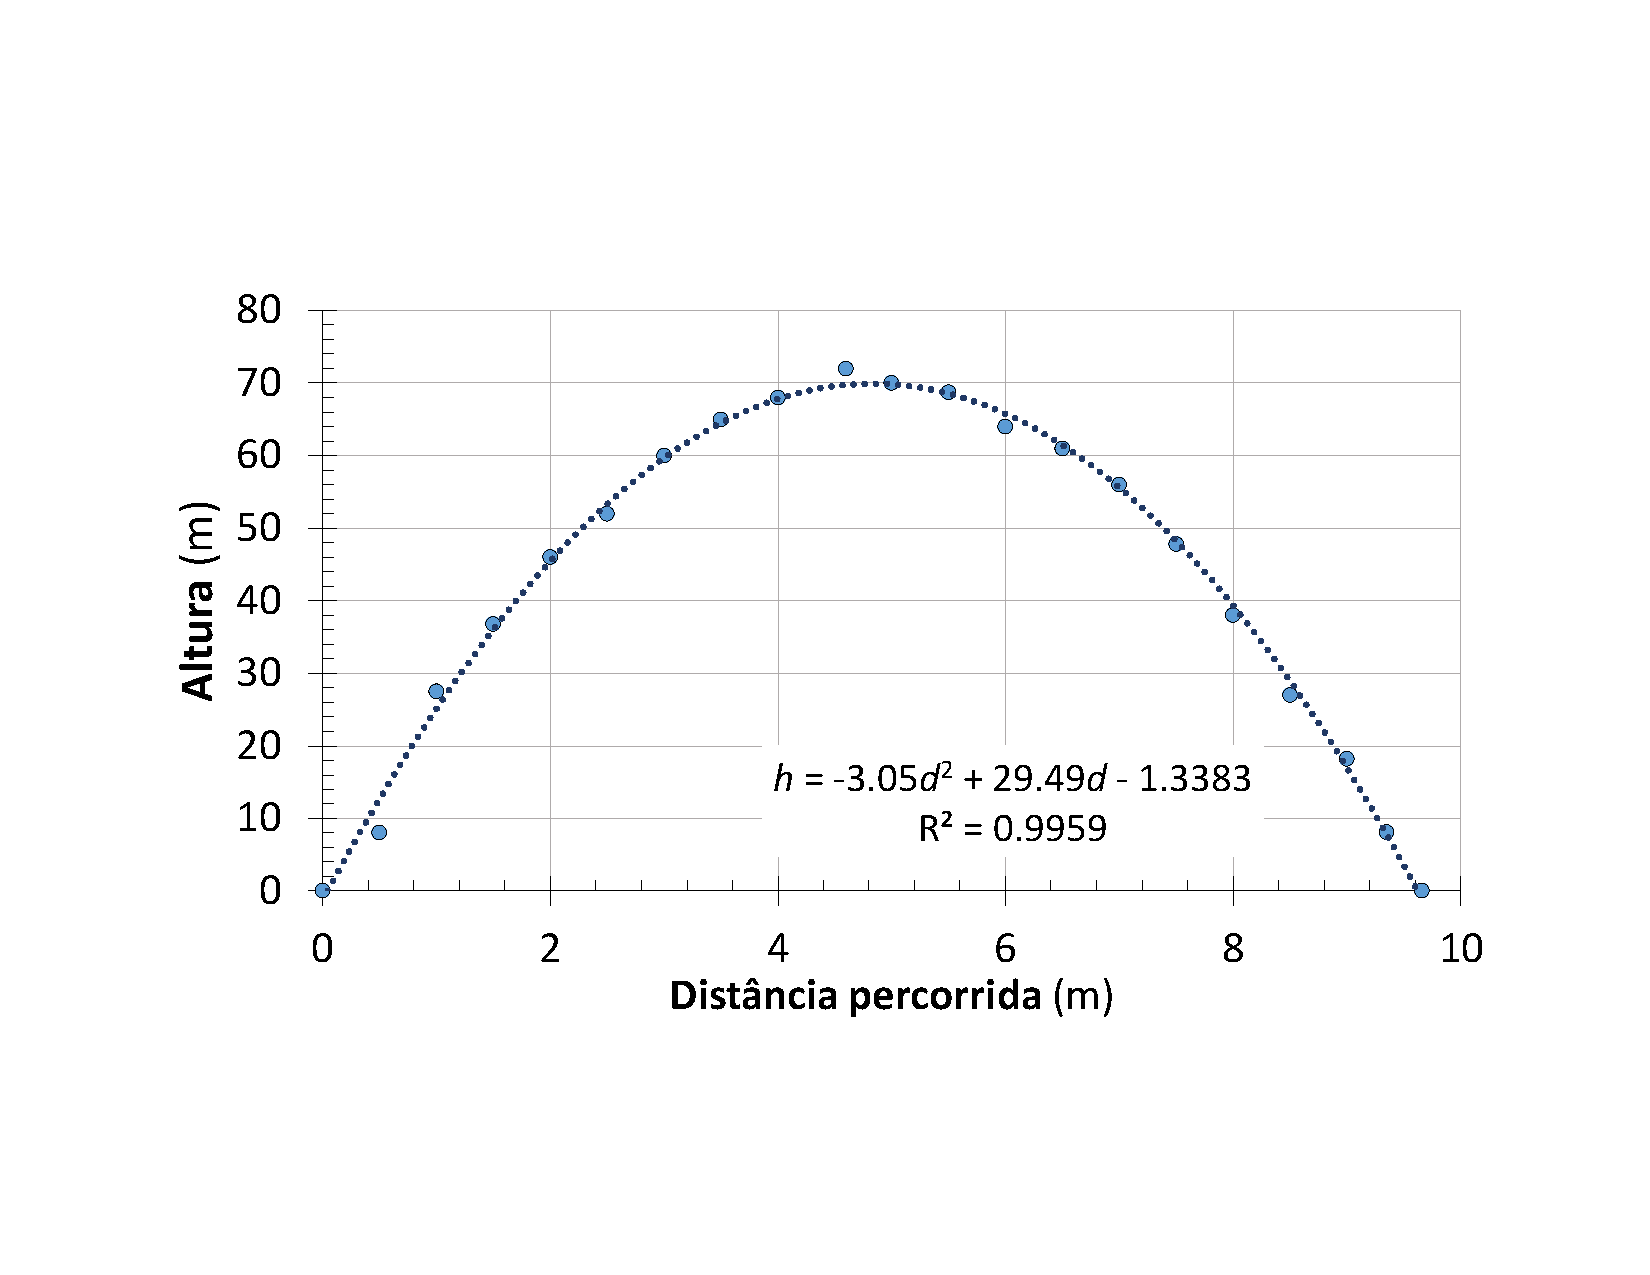
\includegraphics[height=60mm]{cap1/grafico1b.pdf}
	\end{center}
	\vspace{-12pt} % reduz espaço entre figura e caption
	\caption{Gráfico preparado com maior cuidado, incluindo títulos dos eixos
	e unidades}
	\label{fig_grafico1b}
%\end{figure}
%\begin{figure}\sffamily
	\centering
	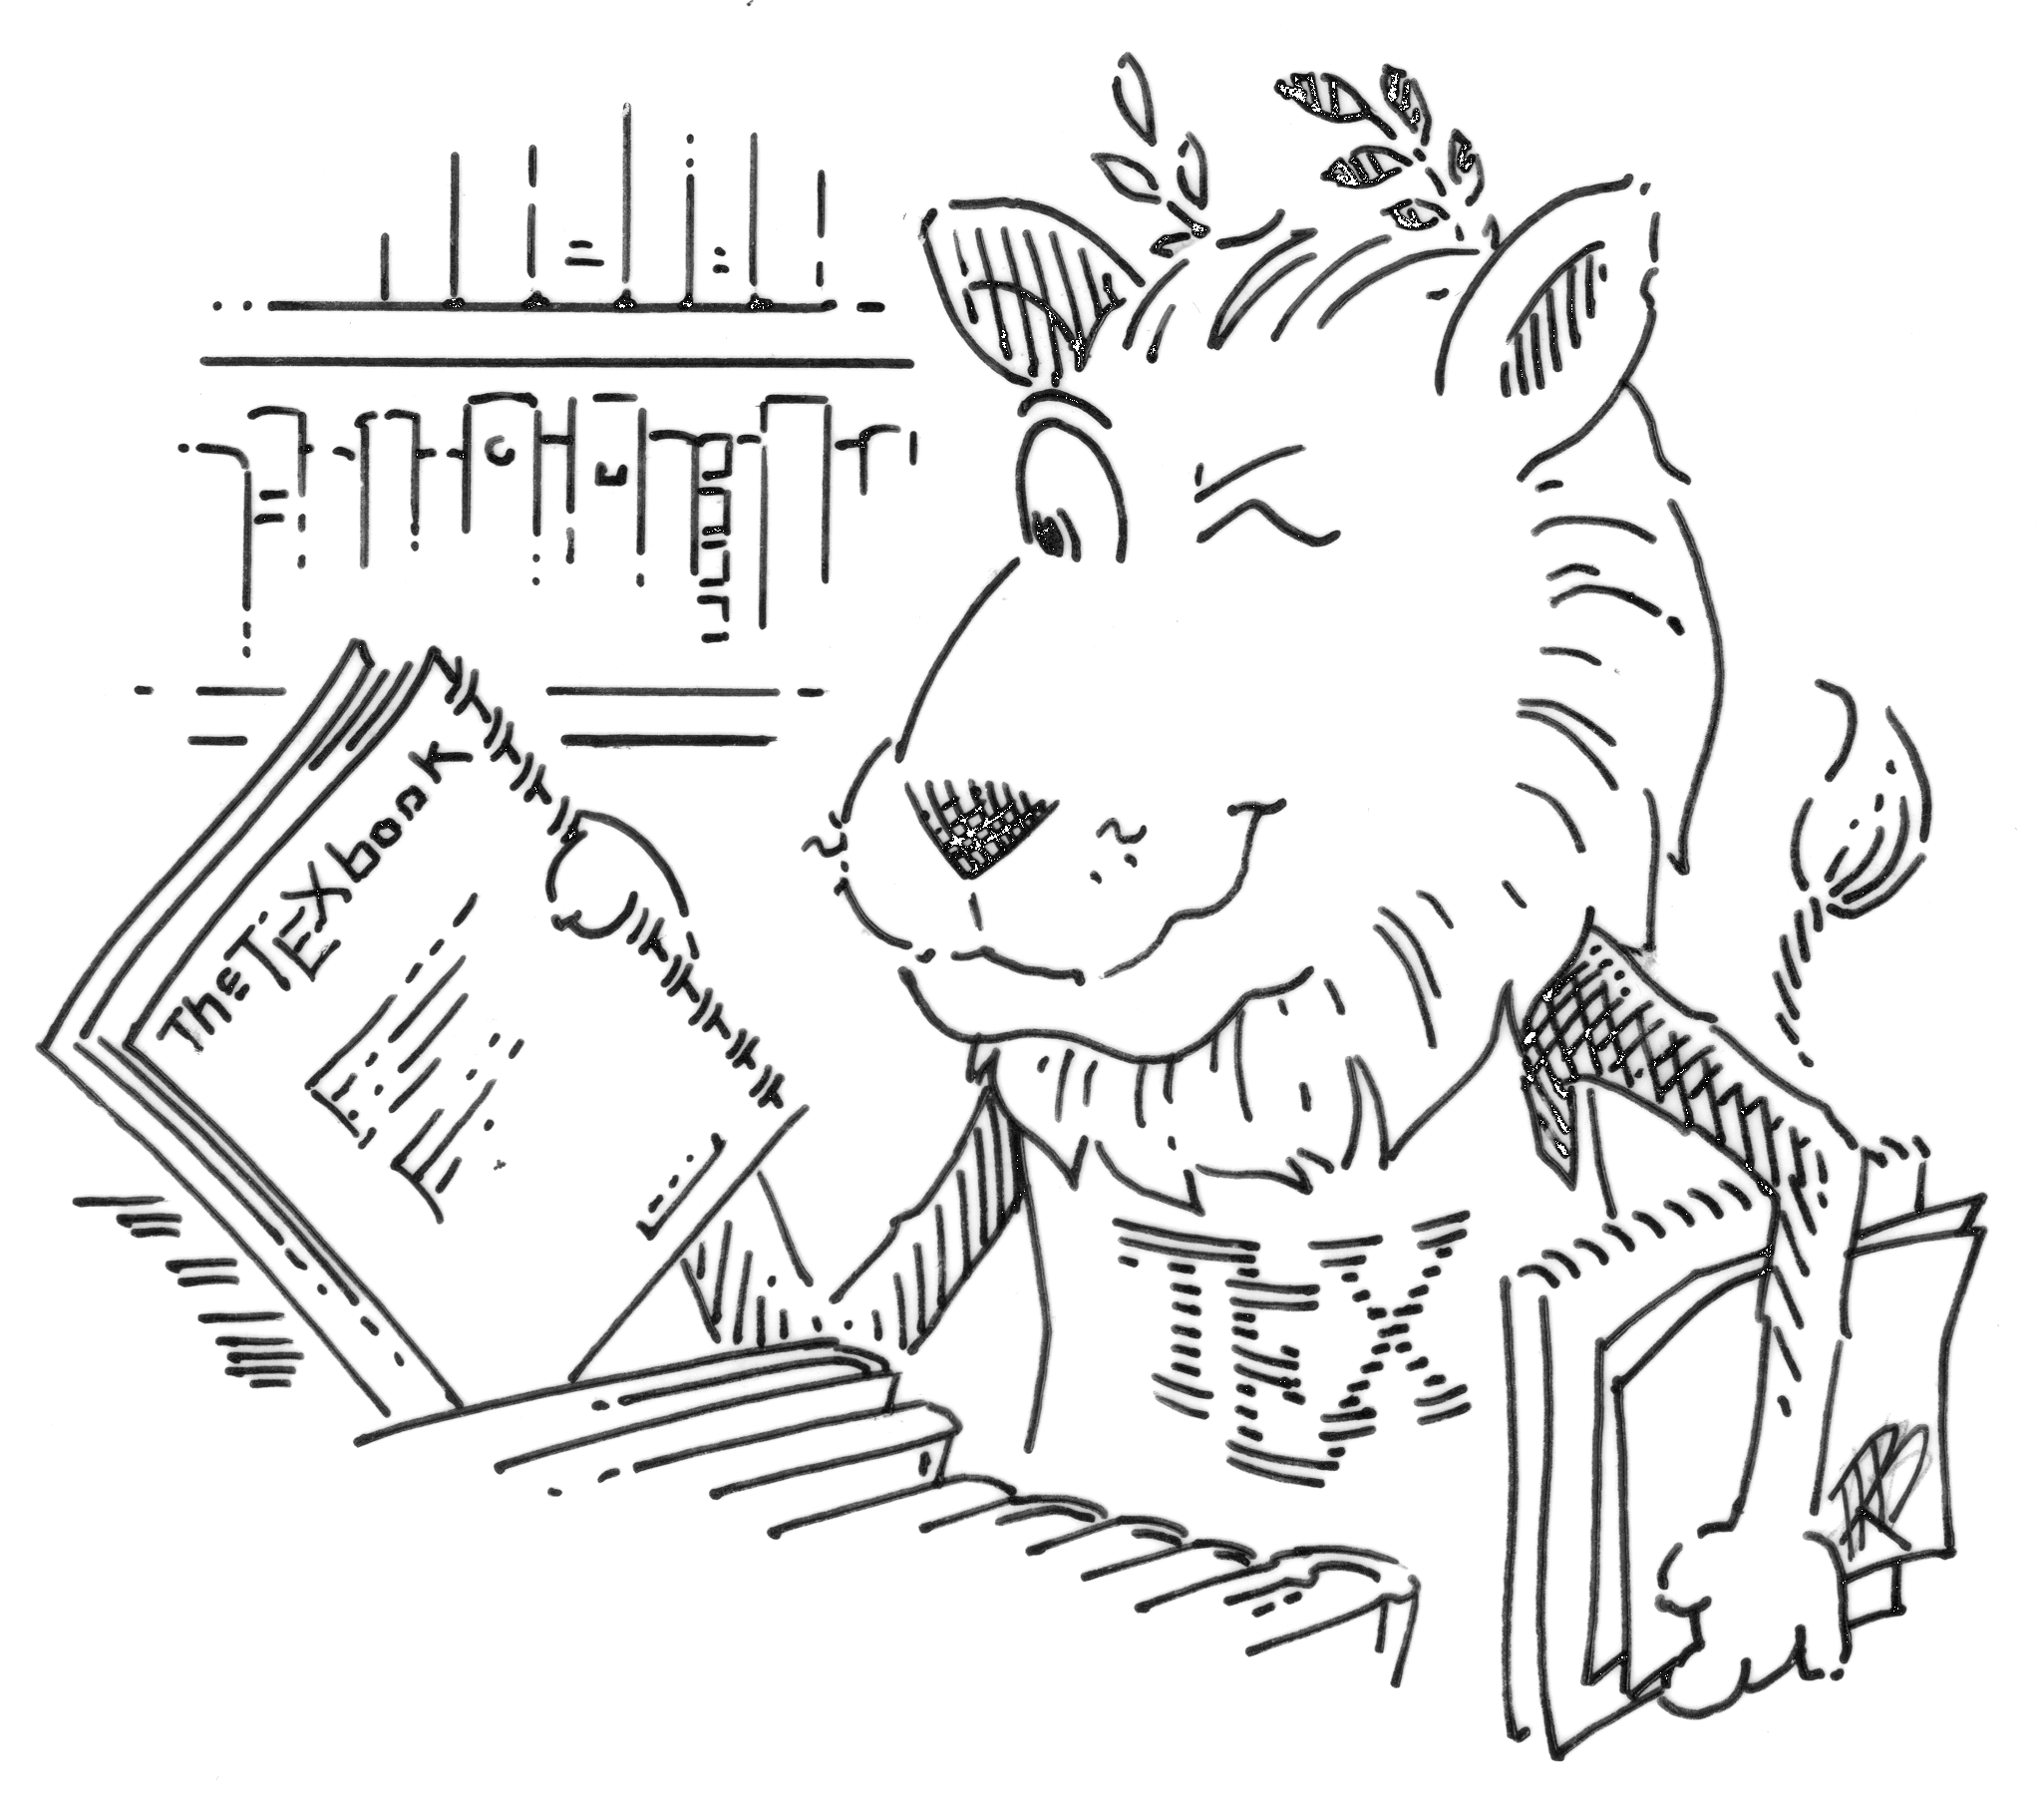
\includegraphics[height=60mm]{cap1/tex_lion_600.png}
	\caption{Arquivos raster do tipo JPEG ou PNG podem
	ser incluido diretamente em figuras}
	\label{f:lion}
\end{figure}



Na \autoref{fig_grafico}, \texttt{abntex2-img-grafico.pdf}  é um  arquivo 
externo, usado no ambiente \texttt{figure}. O gráfico foi elaborado no Excel
e pode-se notar que há um problema com o tamanho das letras, que ficaram
praticamente ilegíveis quando a figura foi reduzida para a largura da página,
160~mm. Com um certo cuidado, é possível criar uma figura bem mais legível, 
como pode visto na \autoref{fig_grafico1b}. 

O ideal é que as letras e números
na figura combinem em aparência com as usadas no texto. Se você 
optar por usar caracteres sem serifa nas tabelas, faça isso para todas elas
e use também os mesmos caracteres sem serifa nas figuras. Procure fazer
com que os caracteres das figuras sejam 10--20\% menores que o do texto, 
lembrando-se de que poderão ser reduzidos para caber na página. Planejando
o tamanho da figura no texto (por ex., 160~mm de largura), é possível escolher
o tamanho dos caracteres no Excel. Na  \autoref{fig_grafico1b}, o tamanho 
original dos caracteres é 12~pt e as dimensões do gráfico gerado pelo Excel são 
$228 \times 126$~mm, com números de 5~mm de altura.


A vantagem de usar imagens vetoriais (como o arquivo \texttt{grafico1b.pdf}) é
que, não importa a escala escolhida (opção \texttt{[width=100mm]}), as figuras
sempre aparecerão com a máxima qualidade. Além disso, os arquivo final do 
texto ficará menor. No entanto, o \LaTeX\ também permite a inclusão de arquivos
raster do tipo \textsc{jpeg} ou  \textsc{png}. A \autoref{f:lion} exemplifica como
inserir um arquivo raster numa figura em \LaTeX\ usando o comando \texttt{%
\textbackslash{}includegraphics[\textrm{\emph{opt}}]\{\textrm{\emph{arq}}\}}.


% ---
\section{Enumerações: comandos do \LaTeX\ e do {abn\TeX{}2}}
% ---

Para a criação de listas, a classe \abnTeX\ fornece os 
ambientes \texttt{alineas}, \texttt{subalineas} e \texttt{incisos}, 
que complementam os ambientes \texttt{itemize}, \texttt{enumerate}
e \texttt{description} do \LaTeX. 

\index{alíneas}\index{subalíneas}\index{incisos} A NBR6024 
 determina que a organização
de assuntos de uma seção que não possuam títulos deve ser
feita através de alíneas \cite[item~4.2]{NBR6024:2012}:

\begin{alineas}
  \item os diversos assuntos que não possuam título próprio, dentro de uma mesma
  seção, devem ser subdivididos em alíneas\footnote{As notas de rodapé devem ficar
  dentro das margens, separadas do texto por um espaço simples entre as
  linhas e por filete de 5 cm, a partir da margem esquerda. Devem ser
  alinhadas, a partir da segunda linha da mesma nota, abaixo da primeira letra
  da primeira palavra, de forma a destacar o expoente, sem espaço entre elas e
  com fonte menor. \citeonline[5.2.1]{NBR14724:2011}}; 
  
  \item o texto que antecede as alíneas termina em dois pontos;
  \item as alíneas devem ser indicadas alfabeticamente, em letra minúscula,
  seguida de parêntese. Utilizam-se letras dobradas, quando esgotadas as
  letras do alfabeto;

  \item as letras indicativas das alíneas devem apresentar recuo em relação à
  margem esquerda;

  \item o texto da alínea deve começar por letra minúscula e terminar em
  ponto-e-vírgula, exceto a última alínea que termina em ponto final;

  \item o texto da alínea deve terminar em dois pontos, se houver subalínea;

  \item a segunda e as seguintes linhas do texto da alínea começa sob a
  primeira letra do texto da própria alínea;
  
  \item subalíneas  são um segundo nível 
  do ambiente \texttt{alineas} e  devem ser conforme as alíneas a
  seguir \cite[item~4.3]{NBR6024:2012}:

  \begin{alineas}
     \item as subalíneas devem começar por travessão seguido de espaço;

     \item as subalíneas devem apresentar recuo em relação à alínea;

     \item o texto da subalínea deve começar por letra minúscula e terminar em
     ponto-e-vírgula. A última subalínea deve terminar em ponto final, se não
     houver alínea subsequente;

     \item a segunda e as seguintes linhas do texto da subalínea começam sob a
     primeira letra do texto da própria subalínea;
     
     \item a classe \abnTeX\ só permite dois níveis do ambiente 
     \texttt{alineas}. 
     
%     \item O terceiro nível deve ser feito com o ambiente
%     \texttt{incisos} e a única diferenciação passa a ser o recuo,
%     pois todos os itens usam o travessão:
%     
%       \begin{incisos}
%    		\item um novo inciso;
%%    		\item mais um nível pode ser criado usando o ambiente 
%%    		\texttt{subalineas}:
%%			  \begin{subalineas}
%%			    \item uma subalínea dentro de um inciso;
%%			    \item uma subalínea usada como um segundo
%%			    nível de \texttt{incisos} (veja o código); 
%%			  \end{subalineas}
%  		\end{incisos}

  \end{alineas}
  
  \item no \abnTeX\ estão disponíveis os ambientes \texttt{incisos} e
  \texttt{subalineas} que, em suma, são o mesmo que se criar outro nível de
  \texttt{alineas}, como nos exemplos à seguir (veja o código):
  
  \begin{incisos}
    \item \textit{um novo inciso em itálico};
    \item ou um inciso sem itálico, que o faz igual a uma subalínea que,
    por sua vez, é um ambiente \texttt{subalineas} dentro de um outro
    \texttt{subalineas};
  \end{incisos}
    
  \item Última alínea com \emph{ênfase}.
  
\end{alineas}

Resumindo, é melhor usar apenas o ambiente \texttt{alineas} quando for
preciso fazer uma lista numerada alfabeticamente; se for preciso fazer
uma sublista dentro desta lista, use \texttt{incisos} ou \texttt{subalineas}
se quiser que ela tenha travessão.

É também possível combinar \texttt{alineas} com \texttt{enumerate} e/ou
\texttt{itemize}, para maior clareza:
  \begin{alineas}
    \item neste caso, \texttt{alineas} faz com o primeiro nível seja enumerado
    	com letras;
    	\begin{enumerate}
    		\item o segundo nível, criado com \texttt{enumerate}, enumera as 
    		alíneas numericamente;
    	\begin{itemize}
    			\item o terceiro nível pode ser criado com \texttt{itemize};
    			\item as alíneas do terceiro nível iniciam-se com um símbolo.
    			\begin{itemize}
    			\item um quarto nível pode ser necessário em alguns casos;
	    			\begin{itemize}
	    			\item um quinto nível pode ser demais;
		    			\begin{itemize}
		    			\item um sexto nível é brincadeira;
		    			\end{itemize} 
	    			\end{itemize} 
    			\end{itemize} 
    		\end{itemize}
    		\item as alíneas do segundo nível começam com um número;
    	\end{enumerate}
    \item uma alínea do primeiro nível inicia-se com uma letra (veja o código); e
    \item a ordem de uso dos ambientes \texttt{alineas}, \texttt{enumerate} e
    \texttt{itemize} pode ser modificada da forma que for mais conveniente para
    a clareza do texto.
  \end{alineas}
Outra forma de organizar as listas poderia ser variando a sequência de ambientes
de lista:
  \begin{enumerate}
    \item neste caso, \texttt{enumerate} faz com o primeiro nível seja enumerado
    	numéricamente;
    	\begin{alineas}
    		\item o segundo nível, criado com \texttt{alineas}, enumera as 
    		alíneas com letras;
    		\begin{incisos}
    			\item o terceiro nível pode ser criado com \texttt{incisos};
    			\item as alíneas do terceiro nível iniciam-se com um travessão. 
    		\end{incisos}
    		\item as alíneas do segundo nível começam com uma letra e parenteses;
    	\end{alineas}
    \item uma alínea do primeiro nível inicia-se com um número (veja o código); e
    \item a ordem de uso dos ambientes \texttt{alineas} e \texttt{enumerate} 
     foi ser modificada para aumentar a clareza do texto.
  \end{enumerate}

% ---
\section{Inclusão de outros arquivos}\label{sec-include}
% ---

É uma boa prática dividir o seu documento em diversos arquivos, e não
apenas escrever tudo em um único. Esse recurso foi utilizado neste
documento. Para incluir diferentes arquivos em um arquivo principal,
de modo que cada arquivo incluído fique em uma página diferente, utilize o
comando:

\begin{verbatim}
   \include{dir/arquivo-a-ser-incluido}      % sem a extensão .tex
\end{verbatim}

Para incluir documentos sem quebra de páginas, utilize:

\begin{verbatim}
   \input{dir/arquivo-a-ser-incluido}      % sem a extensão .tex
\end{verbatim}

% ---
\section{Compilar o documento \LaTeX}
% ---

Geralmente os editores \LaTeX, como o \TeX{}studio ou \TeX{}works
compilam os documentos automaticamente, de modo que você não precisa se
preocupar com isso.




% !TEX encoding = ISO-8859-1

% ---
% Capitulo Genérico
% ---
\chapter[Exemplo de capítulo com um título muito extenso...]
		{Exemplo de capítulo com um título muito extenso em que se explica
		como usar referências bibliográficas}

Este capítulo, cujo título é propositalmente muito extenso, 
apresenta mais alguns comandos específicos da classe \abnTeX\ e 
mostra como incluir referências bibliográficas no texto. O arquivo
\texttt{bib/referencias.bib} contém exemplos dos tipos de referência
mais comuns.

% ---
\section{Divisões do documento: seção}\label{sec-divisoes}
% ---

\LaTeX\ gera a numeração das diversas seções do documento automaticamente. A
classe \abnTeX\ herdou do \LaTeX\ os seguintes comandos para 
dividir o texto em seções, em ordem decrescente de nível:
	\begin{quotation}
	\verb|\part| $\hookrightarrow$ \verb|\chapter| 
	$\hookrightarrow$ \verb|\section| $\hookrightarrow$ \verb|\subsection| 
	$\hookrightarrow$ \\
	$\hookrightarrow$ \verb|\subsubsection| $\hookrightarrow$ \verb|\paragraph| 
	$\hookrightarrow$ \verb|\subparagraph|
	\end{quotation}
Esta seção ilustra o uso de divisões de documentos. \LaTeX\ numera
as seções e subseções até o nível \verb|\subsubsection|. Os níveis
subsequentes não são numerados.

\subsection{Divisões do documento: subseção}\label{subsectA}

Isto é uma subseção. Num texto bem organizado, não é preciso ir além
deste nível de seccionamento numerado, pois a numeração já contém 
três níveis: \ref{subsectA}.

Sed vel dolor a libero dignissim ultrices cursus sed dui. 
Suspendisse sed auctor mi, ac feugiat elit. Aenean in porta lectus, 
nec viverra nisl.


\subsubsection{Divisões do documento: subsubseção}

O nível mais baixo de seções numeradas que você pode usar, no 
\LaTeX, é a \emph{subsubseção}.

  Para encher linguiça, mais texto \emph{dummy}.
  Sed consectetur mauris ipsum, in vehicula lacus viverra vel. 
  Quisque accumsan nulla neque. Nunc dictum mollis dolor ut 
  iaculis. Vivamus aliquam erat nec ante eleifend. 

\subsubsection{Divisões do documento: subsubseção}

Isto é outra subsubseção, o nível mais baixo de seccionamento numerado do texto.
Se você quiser ir além disso, use o comando \verb|\paragraph|.

\paragraph{Subseção de subsubseção}

o comando \verb|\paragraph| não numera a subseção da subsubseção. 

 Para encher linguiça, mais texto \emph{dummy}. Nulla ut nisi 
 vitae tortor molestie pulvinar. Vestibulum sed vehicula nisi. 
 Vivamus sit amet sodales tellus, quis sollicitudin orci.

\subsection{Divisões do documento: subseção}\label{sec-exemplo-subsec}

Isto é uma subseção. Para encher linguiça, mais texto \emph{dummy}. 
Praesent ante mauris, varius blandit pretium eget, blandit ut felis. 
Proin vestibulum ex ac rutrum mattis. Integer ultrices sagittis 
fringilla.

\subsubsection{Divisões do documento: subsubseção}

Isto é mais uma subsubseção da \autoref{sec-exemplo-subsec}.

% ---
\section{Este é um exemplo de nome de seção longo. Ele deve estar
alinhado à esquerda e a segunda e demais linhas devem iniciar logo abaixo da
primeira palavra da primeira linha}
% ---

Isso atende à norma \citeonline[seções de 5.2.2 a 5.2.4]{NBR14724:2011} 
 e \citeonline[seções de 3.1 a 3.8]{NBR6024:2012}.


% ---
\section{Consulte o manual da classe \texttt{abntex2.cls}}
% ---

Consulte o manual da classe \abnTeX\  \cite{abntex2classe} para uma
referência completa das macros e ambientes disponíveis. Além disso, o manual
possui informações adicionais sobre as normas ABNT observadas pelo \abnTeX.
 
% ---
\section{Referências bibliográficas}
% ---

A classe \abnTeX\ usa o pacote \texttt{abntex2cite.sty} para gerar a
bibliografia e as citações bibliográficas ao longo do texto. São dois
os comandos que podem ser usados para fazer citações: 
\verb|\cite{|\emph{rótulo}\verb|}|, para referências implícitas, e 
\verb|\citeonline{|\emph{rótulo}\verb|}|, para referências explícitas.

Uma referência implícita é quando o(s) nome(s) do(s) autor(s) não 
faz(em) parte da sentença, como no exemplo a seguir:\\[6pt]
%\hspace*{1em}%
	{\parbox[t]{6.7cm}{%
	\ttfamily\footnotesize\sloppy
	Valores da aderência \$f\$ variam \\ entre 0,33
	(trilho totalmente limpo \\ e seco) e 0,10, 
	quando o trilho está sujo com óleo 
	\textbackslash{}cite[p.$\sim$82]\{hay82\}.}}
\hspace{\fill} ...que produz...\hspace{\fill}
	{\parbox[t]{5.5cm}{%
	\footnotesize Valores da aderência $f$ variam entre 0,33
	(trilho totalmente limpo e seco) e 0,10, 
	quando o trilho está sujo com óleo 
	\cite[p.~82]{hay82}.}}\\[12pt]
	
Referências implícitas são feitas usando-se o comando 
\verb|\cite{|\emph{rótulo}\verb|}|, em que \emph{rótulo} identifica
o documento bibliográfico a que se faz referência -- no caso do
exemplo, \texttt{hay82}. Os exemplos a seguir mostram casos em que
há mais de um autor:\\[6pt]
	{\parbox[t]{6cm}{%
	\ttfamily\footnotesize
	Uma explicação mais detalhada\\ 
	pode ser encontrada na\\ literatura 
	\textbackslash{}cite[p.$\sim$128]\{kop95\}.}}
\hspace{1em} ...que produz...\hspace{1em}
	{\parbox[t]{6cm}{%
	\footnotesize Uma explicação mais detalhada pode
	ser encontrada na literatura  
	\cite[p.~128]{kop95}.}}\\[12pt]
Quando há três autores, o uso do comando 
\verb|\citeonline{|\emph{rótulo}\verb|}| produz:\\[6pt]
	{\parbox[t]{5.5cm}{%
	\ttfamily\footnotesize
	O fenômeno não ocorre no escuro
	\textbackslash{}cite\{huey03\}.}}
\hspace{1em} ...que produz...\hspace{1em}
	{\parbox[t]{6.5cm}{%
	\footnotesize
	O fenômeno não ocorre no escuro 
	\cite{huey03}}}\\[12pt]
Quando há mais de três autores, \texttt{abntex2cite.sty} usa 
\emph{et~al.}:\\[6pt]
	{\parbox[t]{5.5cm}{%
	\ttfamily\footnotesize
	Esse fenômeno só ocorre no escuro
	\textbackslash{}cite\{huey05\}.}}
\hspace{1em} ...que produz...\hspace{1em}
	{\parbox[t]{6.5cm}{%
	\footnotesize 
	Esse fenômeno só ocorre no escuro
	\cite{huey05}.}}\\[12pt]

Referências explícitas são aquelas em que o(s) nome(s) do(s) autor(s)  
faz(em) parte da sentença. O comando \verb|\citeonline{|\emph{rótulo}\verb|}|
deve ser usado nesses casos, como mostra o exemplo a seguir:\\[6pt]
	{\parbox[t]{5.5cm}{%
	\ttfamily\footnotesize
	Uma explicação mais detalhada\\ 
	pode ser encontrada em\\ 
	\textbackslash{}citeonline[p.$\sim$128]\{kop95\}.}}
\hspace{1em} ...que produz...\hspace{1em}
	{\parbox[t]{6.5cm}{%
	\footnotesize Uma explicação mais detalhada pode
	ser encontrada em  
	\citeonline[p.~128]{kop95}.}}\\[12pt]
Quando há três autores, o uso do comando 
\verb|\citeonline{|\emph{rótulo}\verb|}| produz:\\[6pt]
	{\parbox[t]{5.5cm}{%
	\ttfamily\footnotesize
	\textbackslash{}citeonline\{huey03\}
	discutem o fenômeno sob...}}
\hspace{1em} ...que produz...\hspace{1em}
	{\parbox[t]{6.5cm}{%
	\footnotesize 
	\citeonline{huey03}
	discutem o fenômeno sob...}}\\[12pt]
Quando há mais de três autores, o resultado é mostrado no exemplo
a seguir:\\[6pt]
	{\parbox[t]{5.5cm}{%
	\ttfamily\footnotesize
	\textbackslash{}citeonline\{huey05\}
	é a\\ referência básica do assunto.}}
\hspace{1em} ...que produz...\hspace{1em}
	{\parbox[t]{6.5cm}{%
	\footnotesize 
	\citeonline{huey05}
	é a referência básica do assunto.}}\\[12pt]

\section{A base de dados bibliográficos}

\textsc{Bib}\TeX\ é um programa associado ao \LaTeX\ que usa o pacote \texttt{abntex2cite.sty} e uma base de dados bibliográficos para
construir a bibliografia do documento. A base (ou bases) de dados usada para 
montar a lista de referências bibliográficas é indicada no documento
raiz pelo comando 
\texttt{\textbackslash{}bibliography\{\textrm{\emph{arq\_1,...,arq\_n}}\}},
em que \emph{arq\_i} é um arquivo com extensão \texttt{.bib}, que contém
as dados usados para a montagem das referências bibliográficas. 

Uma entrada do arquivo \emph{arq\_i}\texttt{.bib} tem o seguinte formato
geral:\\
\hspace*{3em}\verb|@tipo{rótulo,|\\
	\hspace*{5em}\verb|dados_obrigatórios [,|\\ 
	\hspace*{5em}\verb|dados_opcionais] }| \\
em que \verb|@tipo| define o tipo da referência 
   			bibliográfica (artigo, livro, tese etc.); 
	\texttt{rótulo} é uma string usada para 
			identificar a referência (como \texttt{setti98a});
	\texttt{dados\_obrigatórios} são os campos de dados que 
   			devem ser fornecidos para possibilitar a construção 
   			da referência pelo \textsc{Bib}\TeX; e
	\texttt{dados\_opcionais} são dados que complementam
     		os obrigatórios. 
Os tipos de referência e os dados, obrigatórios
e opcionais, são descritos no item~\ref{bibtex_entries}, a seguir.

É boa política preencher todos os campos de dados para os quais você
dispõe de informações. Você poderá reusar um arquivo \texttt{.bib} em
qualquer arquivo \texttt{.tex} que você fizer e alguns pacotes 
para montagem de bibliografias podem exigir certos dados além do
mínimo exigido pelo \textsc{Bib}\TeX. Por exemplo,  \texttt{abntex2cite.sty}
irá colocar \emph{[S.l.]} (sem local) em referências nas quais o campo 
\texttt{address} não existir (dependendo do tipo de referência), 
apesar desse campo ser opcional para a maioria dos tipos de referência
previstos no \textsc{Bib}\TeX.


O arquivo 
\texttt{bib/referencias.bib} contém exemplos de elementos bibliográficos
numa base de dados do \textsc{Bib}\TeX.{} Os tipos de referência previstos
pelo \textsc{Bib}\TeX\ incluem:
	\begin{alineas}
		\item livro (\verb|@book|),  \cite{kop95};
		\item capítulo ou trecho de livro (\verb|@inbook|);
		\item artigo em periódico (\verb|@article|) \cite{huey03};
		\item trabalho publicado em anais de congresso 
		(\verb|@inproceedings|);
		\item anais (completos) de congresso (\verb|@proceedings|);
		\item manual (\verb|@manual|) \cite{epslatex06};
		\item tese de doutorado (\verb|@phdthesis|);
		\item dissertação de mestrado (\verb|@mastersthesis|);
		\item relatório técnico (\verb|@techreport|); e
		\item documento que não pode ser classificado em
		nenhum outro tipo (\verb|@misc|).
	\end{alineas}
Além dos listados, que são os mais comuns numa tese ou
dissertação, há muitos outros elementos especificados
no manual do \texttt{abntex2cite.sty}, disponível neste 
\href{http://ctan.math.washington.edu/tex-archive/macros/latex/contrib/abntex2/doc/abntex2cite-alf.pdf}{\fbox{\texttt{link}}}.

O Google Scholar permite exportar referências em formato \textsc{Bib}\TeX,
o que pode facilitar um pouco sua vida, se o tipo e o formato estiverem
corretos (o que nem sempre acontece, na minha experiência).

\subsection{Tipos de referência e dados necessários}
\label{bibtex_entries}

%%----
% Definição de um novo comando, \campo para evitar escrever
%	\hspace*{1em}\texttt{_arg_}: em todos os campos
\newcommand{\campo}[1]{\hspace*{1em}\texttt{#1}:}
%%----
% Define comando \ttz{...} que equivale a \texttt{...}
\newcommand{\ttz}[1]{\texttt{#1}}

A lista a seguir define os tipos de referências previstos no 
\textsc{Bib}\TeX\ e, para cada um deles, quais são os dados 
obrigatórios e os opcionais, explicando como cada campo
deve ser preenchido. Os tipos podem ser escritos em minúsculas
\verb|@tipo| ou maiúsculas \verb|@TIPO|, sem causar problemas. 
Para maiores detalhes sobre os tipos de referências e os campos
de cada tipo consulte este 
\href{http://bib-it.sourceforge.net/help/fieldsAndEntryTypes.php}
{\fbox{\texttt{link}}}.
\begin{alineas}

	\item \verb|@BOOK| -- se a referência for um livro publicado por uma
		editora (use \verb|@inbook| para capítulo ou trecho de livro) \\
		\emph{Campos obrigatórios:}\\
 			\campo{author [ou] editor} nome do autor ou do editor;\\
 			\campo{title} título do livro;\\
 			\campo{publisher} nome da editora que publicou o livro; e \\
 			\campo{year} ano da publicação.\\
		\emph{Campos opcionais}:\\
			\campo{volume} número do volume, se houver mais de um; \\
			\campo{series} número do livro, se fizer parte de uma série;\\
 			\campo{address} cidade de publicação (evite omitir este campo);\\
 			\campo{edition} número da edição, se não for a única;\\
 			\campo{month} mês de publicação;\\
 			\campo{note} qualquer observação desejada; \\
 			\campo{key} usado para ordenação alfabética e citação, se
 				\texttt{author} e \texttt{editor} não existem.\\
		\emph{Exemplos em \texttt{bib/referencias.bib}:} \\
			\hspace*{1em}\citeonline{hay82} e \citeonline{kop95} ou 
			\cite{hay82,kop95,epe13,epe13b}\\
		\emph{Observações:} Não confundir \texttt{key}
 				com \texttt{rótulo}, que é usado para identificar a 
 				referência para o \textsc{Bib}\TeX. \texttt{key} não
 				é usado por \texttt{abntex2cite.sty}, por causa da 
 				norma da ABNT. Para livros sem autor e editor, eu sugiro 
 				verificar os dados de \citeonline{epe13}, para evitar
 				algo assim: \citeonline{epe13b} -- os dois são o
 				mesmo livro.
 				
	\item \verb|@INBOOK| -- capítulo ou parte de um livro (veja 
		\verb|@incollection| para outro caso de parte de livro) \\
		\emph{Campos obrigatórios:}\\
 			\campo{chapter [ou] pages} número do capítulo ou das páginas 
 			  citadas;\\
 			\texttt{author} ou \texttt[editor]; \texttt{title}; 
 			\texttt{publisher}; e \ttz{year}.\\
		\emph{Campos opcionais}:\\
			\texttt{volume}; \texttt{series}; \texttt{address};
			\texttt{edition};\texttt{month}; \texttt{note}\\
		\emph{Exemplos em \texttt{bib/referencias.bib}:} \\
			\hspace*{1em}\citeonline{kop95c3} ou 
			\cite{kop95c3,epe13a} 
	\emph{Observações:} O resultado fica ruim nos dois casos.
			Não dá para usar com o \texttt{abntex2cite.sty}.
		
	\item \verb|@INCOLLECTION| -- capítulo ou parte de um livro com
		seu próprio título e autor \\
		\emph{Campos obrigatórios:}\\
 			\campo{booktitle}  título do livro;\\
 			\campo{title} título do capítulo; \\
 			\campo{author} autor do capítulo; \\
 			\texttt{publisher}; e \ttz{year}.\\
		\emph{Campos opcionais}:\\
			\texttt{editor}; \texttt{volume [ou] número}; 
			\texttt{series}; \texttt{address};
			\texttt{edition};\texttt{month}; \texttt{note}\\
		\emph{Exemplos em \texttt{bib/referencias.bib}:} \\
			\hspace*{1em}\citeonline{cop05c2,cope2005} 
			\cite{cop05c2,cope2005}
		\emph{Observações:} O resultado fica ruim nos dois casos, 
			coloca-se o título do livro no lugar do título do 
			do capítulo. Não dá para usar com o \texttt{abntex2cite.sty}. 
			Veja como colocar sobrenomes compostos com \emph{Junior}, 
			\emph{Neto} e \emph{Filho} para que saiam corretamente
			no texto e na bibliografia. 

		\item \verb|@ARTICLE| para um artigo publicado num periódico
			científico ou numa revista\\
		\emph{Campos obrigatórios:}\\
 			\campo{journal}  nome do periódico;\\
 			\hspace*{1em}\ttz{title}; \ttz{author}; e \ttz{year}.\\
		\emph{Campos opcionais}:\\
			\hspace*{1em}\texttt{volume}; \texttt{number}; 
			\texttt{pages}; \texttt{month}; e \texttt{note}\\
		\emph{Exemplos em \texttt{bib/referencias.bib}:} \\
			\cite{huey03}
			
	\item \verb|@INPROCEEDINGS| trabalho publicado nos anais de
			um congresso científico\\
		\emph{Campos obrigatórios:}\\
 			\campo{booktitle}  título dos anais do congresso;\\
 			\hspace*{1em}\ttz{title}; \ttz{author}; e \ttz{year}.\\
		\emph{Campos opcionais}:\\
			 \hspace*{1em}\ttz{editor}; \ttz{volume}; \ttz{number}; \ttz{series}; 
			 \ttz{address}; 
			\texttt{pages}; \texttt{month}; \ttz{organization};\\
			\hspace*{1em}\ttz{publisher} e \texttt{note}\\
		\emph{Exemplos em \texttt{bib/referencias.bib}:} \\
			\cite{mil2009}, \citeonline{mil2009} e \cite{aut:06} \\
		\emph{Observações:} Os sobrenomes ``de Mileto'' e ``von Samos''
		são tratados corretamente se ``de'', ``von'' ou ``da'' estiverem
		em minúsculas. Use o campo \ttz{note} para incluir
		coisas como ``(CD-ROM)'' ou a url dos anais do congresso. 
		\citeonline{aut:06} é um exemplo de citação cruzada
		(veja \ttz{aut:06} e \ttz{conf:06} no arquivo \ttz{.bib}). 
			
			
	\item \verb|@PROCEEDINGS| para citar os anais de um congresso
			científico (o livro todo)\\
		\emph{Campos obrigatórios:}\\
 			\hspace*{1em}\ttz{title} e \ttz{year}.\\
		\emph{Campos opcionais}:\\
			 \hspace*{1em}\ttz{editor}; \ttz{volume}; \ttz{number}; 
			 \ttz{series}; \ttz{address}; \texttt{month}; \ttz{organization};\\
			\hspace*{1em}\ttz{publisher} e \texttt{note}\\
		\emph{Exemplos em \texttt{bib/referencias.bib}:} \\
			\citeonline{conf:06} e \cite{conf:06} \\
			
	\item \verb|@MANUAL| normalmente, manual de um software (veja
		\ttz{techreport} \\
		\emph{Campos obrigatórios:}\\
 			\hspace*{1em}\ttz{title}.\\
		\emph{Campos opcionais}:\\
			 \hspace*{1em}\ttz{author};   \ttz{organization};
			 \ttz{edition}; \ttz{address}; \texttt{month};
			\ttz{year} e \texttt{note}\\
		\emph{Exemplos em \texttt{bib/referencias.bib}:} \\
				\citeonline{epslatex06}, \cite{epslatex06}

	\item \verb|@TECHREPORT| um relatório técnico, publicado por
		uma organização, com ou sem autor, às vezes numerado numa
		série \\
		\emph{Campos obrigatórios:}\\
 			\hspace*{1em}\ttz{title}; \ttz{author}; \ttz{institution}
 			e \ttz{year}\\
		\emph{Campos opcionais}:\\
			 \hspace*{1em}\ttz{type};   \ttz{number};
			 \ttz{address}; \texttt{month};
			e \texttt{note}\\
		\emph{Exemplos em \texttt{bib/referencias.bib}:} \\
				\citeonline{gomez03} (\ttz{gomez03}), \cite{dnit06}
				(\ttz{dnit06})
		\emph{Observações:} Veja que não aparece nem o tipo de relatório
		nem seu número -- mais um problema do \ttz{abntex2cite.sty}. Em 
		\ttz{gomez03} não aparece o nome da instituição. Melhor evitar
		este tipo no \ttz{abntex2cite.sty}.	Tente \ttz{misc}.		
								
	\item \verb|@PHDTHESIS| uma tese de doutorado \\
		\emph{Campos obrigatórios:}\\
 			\hspace*{1em}\ttz{author}; \ttz{title}; \ttz{school}; e \ttz{year}.\\
		\emph{Campos opcionais}:\\
			 \hspace*{1em}  \ttz{type};
			 \ttz{address}; \texttt{month};
			 e \texttt{note}\\
		\emph{Exemplos em \texttt{bib/referencias.bib}:} \\
				\citeonline{cunha13}, \cite{cunha13}
	
	\item \verb|@MASTERSTHESIS| uma dissertação de mestrado \\
		\emph{Campos obrigatórios:}\\
 			\hspace*{1em}\ttz{author}; \ttz{title}; \ttz{school}; e \ttz{year}.\\
		\emph{Campos opcionais}:\\
			 \hspace*{1em}  \ttz{type};
			 \ttz{address}; \texttt{month};
			 e \texttt{note}\\
		\emph{Exemplos em \texttt{bib/referencias.bib}:} \\
				\citeonline{cunha09}, \cite{cunha09}
					
	\item \verb|@misc| um documento genérico, que pode resolver
		alguns dos seus problemas \\
		\emph{Campos obrigatórios:}\\
 			\hspace*{1em}nenhum\\
		\emph{Campos opcionais}:\\
			 \hspace*{1em}\ttz{author}; \ttz{title}; 
			 \ttz{howpublished}; \texttt{month}; \ttz{year};
			 e \texttt{note}\\
		\emph{Exemplos em \texttt{bib/referencias.bib}:} \\
				\citeonline{oli87} e \cite{oli87} e, para um documento na
				web: \cite{epsl}. Teste para ver se fica certo 
				\cite{epsl, epslatex06}.
			
\end{alineas}




% ---
% Finaliza a parte no bookmark do PDF, para que se inicie o bookmark na raiz
% ---
\bookmarksetup{startatroot}% 
% ---

% ---
% Conclusão
% ---
% !TEX encoding = ISO-8859-1

\chapter{Conclusões}

Lendo os arquivos \ttz{.tex} usados para produzir este documento, você
poderá ver alguns exemplos de como \LaTeX\ foi usado para obter o
resultado desejado. Tenha em mente que as soluções usadas não
são as únicas formas de produzir aqueles resultados~--~considere-as
meros exemplos do que pode ser feito com \LaTeX. 

Conforme seu
conhecimento de \LaTeX\ for aumentando, você será capaz de 
inventar suas próprias soluções ou aperfeiçoar as soluções
criadas por outras pessoas. Por isso, tenha sempre à mão
um boa referência de \LaTeX, como \citeonline{kop2004}.
Outras boas fontes de informações sobre \LaTeX\ são 
\href{http://tex.stackexchange.com/questions}{\fbox{\ttz{tex.stackexchange.com/questions}}} e
\href{http://www.latex-community.org/forum/}{\fbox{\ttz{latex-community.org/forum}}} --
pois é muito comum que alguém já tenha tido o mesmo problema antes e 
algum \TeX{}pert tenha sugerido como resolvê-lo num desses fóruns. 

% ----------------------------------------------------------
% ELEMENTOS PÓS-TEXTUAIS
% ----------------------------------------------------------
\postextual

% ----------------------------------------------------------
% Referências bibliográficas
%
% 	abntex2 usa o estilo abntex2cite para formatação
%	das referências. Leia o capítulo 2 deste documento
%	para mais informações
% ----------------------------------------------------------
\bibliography{bib/referencias,bib/abntex2-modelo-references}

% ----------------------------------------------------------
% Glossário -- elemento opcional, só inclua se necessário
%
%	Nota:	No PPG-ET não é usual colocar um glossário
%			em teses e dissertações. Se for usar, é preciso
%			descomentar as linhas apropriadas
% ----------------------------------------------------------
%
%\glossary

% ----------------------------------------------------------
% Apêndices
%
% Os apêndices, se existirem, devem ser incluídos pelo 
% ambiente \begin{apendicesenv}...\end{apendicesenv}
%	Nota: apêndices são numerados com letras maiúsculas: A, B, ...
%
% ----------------------------------------------------------
% Para incluir um apêndice, descomente as linhas a seguir
%
%\begin{apendicesenv}% Inicia os apêndices
%
%	\partapendices% Imprime uma página indicando o início dos apêndices
%
%	\include{cap_ap/apendice_A}% inclui o apendice A
%	\include{cap_ap/apendice_B}% inclui o apendice B e assim por diante
%
%\end{apendicesenv}% fim dos apêndices

% ----------------------------------------------------------
% Anexos
%
% Anexos, caso existam, devem ser incluídos através do 
% ambiente \begin{anexosenv}...\end{anexosenv}
% 	Nota: anexos são numerados com algarismos arábicos: 1, 2, ...
%
% ----------------------------------------------------------
% Para incluir um ou mais anexos, descomente as linhas a seguir
%
%\begin{anexosenv}% Inicia os anexos
%
%	\partanexos % Imprime uma página indicando o início dos anexos
%
%		\include{cap_anx/anexo_1}% inclui o anexo 1
%
%\end{anexosenv}% fim dos anexos


\end{document}% fim do arquivo raiz da tese/dissertação


